Hlasovací lístek je na straně klienta (voliče) reprezentován formulářem. Tento formulář je generován v Nette na základě specifikací nastavených pro dané volby. Každý hlasovací lístek musí obsahovat nejméně jednu otázku. Otázka obsahuje několik odpovědí a limit pro nejmenší a největší povolený počet zvolených odpovědí. Otázka může být také označena jako povinná.

Z výše uvedeného vyplývá, že formulář je potřeba validovat - zjistit, že odpovědi uvedené na hlasovacím lístku odpovídají specifikacím voleb. Nette umožňuje pravidla validace nastavit již při vytváření formuláře a po jeho odeslání klientem je formulář zvalidován na straně serveru. Neúspěšná validace přeruší zpracování formuláře a~klientovi poskytne zpětnou vazbu (chybové zprávy). Pokud je načtena JavaScriptová knihovna \texttt{netteForms.js}, provádí se validace navíc i na straně klienta~\cite{NetteForms}.

Pokud by byl hlasovací lístek odeslán serveru k validaci, byla by narušena anonymita voleb. A to i v případě, že by server jen ověřil, že počet odpovědí odpovídá nastaveným limitům. Data by server měl k dispozici nešifrovaná a stejně tak identitu voliče, kdokoli by mohl vznést oprávněnou námitku, že takto není zaručena absolutní anonymita voliče. Validace formuláře z tohoto důvodu probíha pouze na straně klienta - v prohlížeči.

Ve fragmentu \ref{php:validaceSkripty} jsou vidět skripty a balíčky, které jsou využívány pro validaci a šifrování hlasovacích lístků na straně klienta. Třída \texttt{Crypto} obsahuje metody pro šifrování dat a komunikaci se serverem za účelem výměny klíčů. Z tohoto důvodu jsou ji předávány odkazy na signály presenteru.

\begin{listing}[ht]
\htmlsnippet{tex/code/votingScripts.html}
\caption{JavaScript použitý při hlasování}
\label{php:validaceSkripty}
\end{listing}

\clearpage
\n{2}{Validace}\label{section:hlasovaniValidace}
Validace formuláře na straně klienta je všeobecně považována za pouhé usnadnění pro uživatele, umožňuje rychle a přehledně uživatele informovat o nesrovnalostech ve~formuláři. Nicméně, veškerá data přijatá od klienta (prohlížeče) by měla být považována za potenciálně nebezpečná a nevalidní, jelikož upravit data před odesláním nebo upravit JavaScriptové validační skripty není nemožné \cite{Sklar2018}\cite{Validace1}\cite{Validace2}\cite{Validace3}.

Je nutné tedy počítat s tím, že data jsou validována již na straně klienta, ale pouze pro potřeby voliče - aby mu byly přehledně komunikovány jakékoli chyby, kterých se během vyplňování hlasovacího lístku dopustil. Na server se data dostanou zašifrována a nebylo by již možné ověřit jejich platnost. To by mohlo snadno vyústit ve vysoké procento neplatných hlasů a v horším případě četným námitkám proti platnosti voleb samotných. Nutnost validovat data na straně serveru nicméně zůstává, pouze se odkládá~na dobu, kdy budou data serverem čitelná - sčítání hlasů.

Po vyplnění formuláře a kliknutí na potvrzovací tlačítko následuje série dílčích kroků, které vedou k odeslání zašifrovaného hlasovacího lístku nebo výpisu chybových hlášení.

\begin{figure}[h]
	\centering
	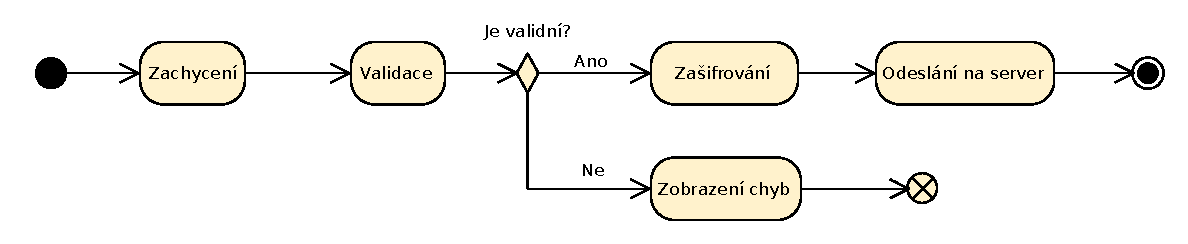
\includegraphics[width=\linewidth]{svg/validace.eps}
	\captionsetup{width=\linewidth}
	\caption[Diagram aktivity validace]{Diagram aktivity validace (zdroj: vlastní)}
	\label{fig:diagramValidace}
\end{figure}

Formulář má nastaveno odesílání pomocí AJAX, událost odeslání formuláře je tedy nejprve zachycena knihovnou Naja. V šabloně je do Naja registrováno rozšíření \texttt{ValidateVotingForm}, což je jedno z vlastních rozšíření zahrnutých v soubrou \texttt{Naja.ext.js}.

Všechna potřebná pravidla pro validaci jsou již nastavena v Nette při generování formuláře a klient má načtenou knihovnu pro validaci formulářů od Nette, k validaci je tedy použita tato knihovna. Bohužel prezentace chyb touto knihovnou není uživatelsky nejpřívětivější, bylo tedy zvoleno validování jednotlivých elementů formuláře samostatně. Pomocí \texttt{HTMLSelectElement.setCustomValidity()} je nevalidním prvkům změněn stav validity, který využívá framework \textit{Bootstrap} \cite{Bootstrap} k~zobrazení validovaného formuláře (pomocí pseudoelementů \texttt{:valid} a \texttt{:invalid}). V~případě, že formulář obsahuje nevalidní prvky, je zobrazena chybová zpráva, zvýrazněny chybné elementy a proces ukončen.

\begin{listing}[ht]
\jssnippet{tex/code/validace.js}
\caption{část třídy ValidateVotingForm}
\label{php:validace}
\end{listing}

\n{2}{Šifrování}
Data zvalidovaného formuláře jsou uspořádána do asociativního pole a předána k~zašifrování třídě \texttt{Crypto}. Tato třída má ze šablony předány odkazy pro komunikaci se serverem a již po svém instanciování si od serveru vyžádá veřejný klíč volební komise a veřejný podpisový klíč serveru (oba RSA) a vygeneruje nový náhodný klíč AES-GCM (256-bit) a \textit{nonce} (inicializační vektor). Jednotlivé operace jsou prováděny asynchronně na pozadí, uživatele tedy nijak neomezují.

Ve chvíli, kdy je hlas předán třídě Crypto, je volební lístek (pole) převeden na~JSON řetězec a zašifrován pomocí vygenerovaného AES klíče. Díky použité metodě šifrování je výsledný šifrovaný text pro stejný otevřený text pokaždé jiný. Následně je zašifrován i samotný AES klíč, a to RSA klíčem volební komise (s RSA-OAEP výplní). Dále je na~sha-256 hash šifrovaného klíče aplikován náhodný faktor zaslepení $r$ podle algoritmu popsaného v části \ref{section:blindSign}. Zaslepená zpráva je odeslána na server k podpisu.

Server přijímá zaslepenou zprávu, která neobsahuje žádné informace o hlasovacím lístku, jedná se pouze o hash klíče použitého k zašifrování hlasovacího lístku. Aby bylo možné na straně klienta z podepsané zprávy odstranit náhodný faktor $r$, není možné použít žádné výplně. Použitá knihovna \texttt{phpseclib} navíc jako dodatečnou ochranu podpisového klíče proti časovým útokům používá zaslepování \cite{phpseclibBlinding}, které by rovněž znemožnilo odstranění faktoru $r$, proto nebylo použito. Podepsaná zpráva je vrácena zpět klientovi k dalšímu zpracování.

Na straně klienta je z podepsané zprávy odstraněn náhodný faktor $r$ reverzní operací zaslepení. Tím je získán validní podpis původní (nezaslepené) zprávy - zašifrovaného AES klíče. Pomocí veřejného podpisového klíče serveru a hashe zašifrovaného AES klíče je ověřena správnost podpisu. Pokud podpis zprávy odpovídá originálu, na server se odešle k uložení zašifrovaný hlasovací lístek, zašifrovaný AES klíč a podpis.

%\obr{Sekvenční diagram šifrování}{fig:diagramSifrovani}{0.6}{svg/sifrovani.eps}
\begin{figure}[h]
	\centering
	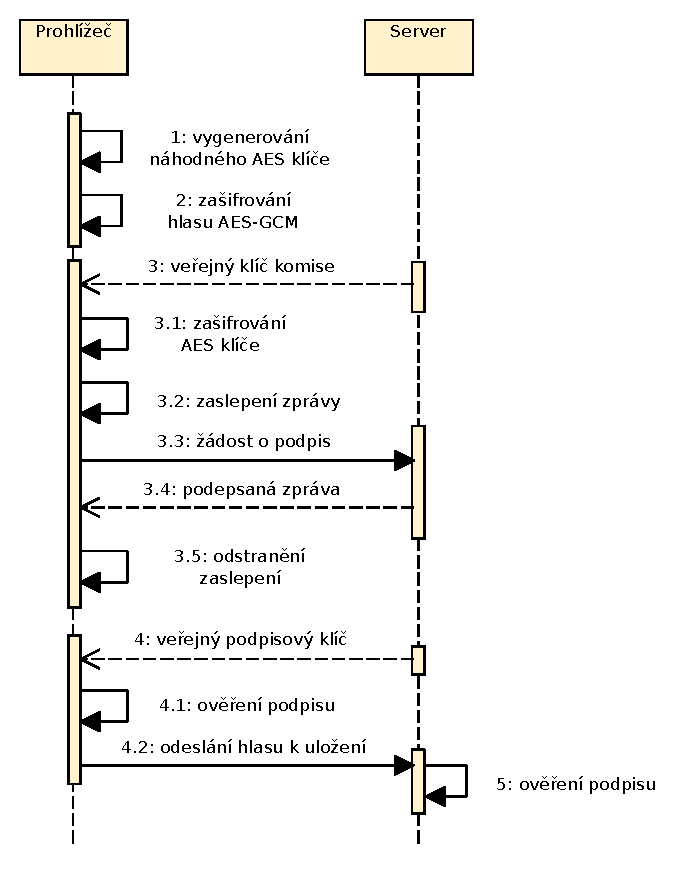
\includegraphics[width=0.8\linewidth]{svg/sifrovani.eps}
	\captionsetup{width=0.8\linewidth}
	\caption[Sekvenční diagram šifrování]{Sekvenční diagram šifrování (zdroj: vlastní)}
	\label{fig:diagramSifrovani}
\end{figure}

\n{2}{Ukládání}

V tuto chvíli se nabízí dotaz, proč aplikovat slepé podepisování, když server, který vystavuje podpis, zároveň zpracovává originál zprávy, kterou podepsal. Tento způsob byl zvolen s ohledem na univerzálnost použití. Právě díky slepému podepisování může být k ukládání hlasů použit jiný server zcela nezávislý na zbytku systému. Tento nezávislý server si pomocí veřejného podpisového klíče ověří, že podpis odpovídá obdržené zprávě a ta je tedy důvěryhodná. Vzhledem k tomu, že se podepisuje pouze hash, je možné připojit i samotná data hlasovacího lístku, nezávislý server by tedy přijímal pouze zprávu a její podpis. Není to nicméně nutností, protože zašifrovaná data mohou být dešifrována pouze jedním klíčem a ten je ověřený volebním serverem.

Po přijetí dat k uložení tedy server opět ověří, že přijatý zašifrovaný AES klíč odpovídá podpisu, který ho provází. Následně vytvoří entitu \texttt{EncryptedBallot}, nastaví ji přijatá data a předá repozitáři k uložení. Zároveň je u voliče zaznamenán čas, kdy hlasoval, aby bylo možné zamezit opakovanému hlasování, pokud ve stejných volbách již svůj hlas odevzdal. Jak bylo řečeno výše, ověření a uložení přijatých dat může provést i jakákoli důvěryhodná třetí strana, volební server pouze potřebuje vědět, že volič úspěšně hlasoval.

\n{2}{Sčítání}
Sčítání hlasů je umožněno pouze po skončení voleb, a to uživatelům s patřičným oprávněním. Před sečtením hlasů je nutné je nejdříve dešifrovat, za tímto účelem musí člen volební komise serveru zpřístupnit privátní RSA klíč odpovídající klíči, který byl nahrán volební komisí před začátkem voleb. Z důvodu co nejvyšší možné důvěryhodnosti volebního systému bylo zvoleno řešení, kdy server (nebo kdokoli s~přístupem k němu) nemá možnost hlasy dešifrovat dříve než volební komise uvolní potřebný RSA klíč. Tento způsob ovšem předpokládá správné vygenerování a~bezpečné uložení klíče volební komisí.

Při nahrávání veřejné části RSA klíče je kontrolováno, jestli se jedná o veřejný RSA klíč, který aplikace dokáže použít. Zodpovědnost za poskytnutí správného klíče je ovšem na volební komisi. Pokud by byl poskytnut například klíč, jež je chráněn heslem, aplikace by v současné verzi hlasy nedokázala dešifrovat. Zároveň není umožněno vyzkoušet kompatibilitu veřejného a privátního klíče s aplikací, aby server nepřišel do kontaktu s privátním kíčem dříve než je to absolutně nezbytné.

Pro volby s ukončeným hlasováním je v backendové části aplikace zpřístupněna volba nahrání privátního klíče a v záložce výsledků také tlačítko pro sečtení hlasů. Kliknutí na tlačítko vede na signál \texttt{countBallots}. Proces sčítání hlasů řídí třída \texttt{BallotCounter}, která je závislostí \texttt{ElectionPresenter}. Jediná veřejná metoda této třídy je \phpinline{processBallots($election): array}%$
, která deleguje dešifrování a validaci hlasovacích lístků na třídy \texttt{BallotDecryptor} a \texttt{BallotValidator} a samotné sečtení hlasů provádí sama. Jednotlivé metody této třídy jsou vidět v příloze \ref{priloha:fragmenty}.

Třída \texttt{BallotDecryptor} obsahuje dvě veřejné metody volané z třídy \texttt{BallotCounter}, metoda \phpinline{setElection()} pouze nastaví aktuálně zpracovávané volby a \phpinline{decryptBallots()} nejprve načte zašifrované hlasovací lístky z repozitáře, následně metodou \phpinline{verify($ballot)} %$
 ověří, že hash a podpis uložené v databázi odpovídá zpracovávanému volebnímu lístku a nakonec dešifruje AES klíč, kterým dešifruje samotná data. Dešifrovaná data jsou poté nastavena novému objektu \phpinline{DecryptedBallot}, který je repozitářem uložen. V případě chyby při ověřování, dešifrování a dalších, je chyba zaznamenána do logu (souboru) včetně identifikace hlasovacího lístku. Kód dešifrování je vidět v příloze \ref{priloha:fragmenty}.
  
Třída \texttt{BallotValidator} má za úkol ověřit, že všechny dešifrované hlasovací lístky jsou platné a splňují pravidla nastavená pro dané volby. V zásadě se jedná o pozdní validaci hlasovacího formuláře na straně serveru, jak bylo popsáno v části \ref{section:hlasovaniValidace}. Tato třída obsahuje identické metody jako \texttt{BallotDecryptor} pro nastavení voleb a zpracování lístků. Z~repozitáře jsou získány všechny dešifrované volební lístky a postupně ověřena data v~nich obsažená, že splňují nastavená kritéria. Jmenovitě, že identifikátor voleb souhlasí s aktuálně zpracovávanými a že povinné otázky jsou zodpovězeny a všechny otázky splňují limity pro minimální a maximální počet odpovědí. Kód validace je vidět v příloze \ref{priloha:fragmenty}.

\n{2}{Výsledky}
Výstupem validace jsou tři pole volebních lístků - platné, neplatné a chybné. Neplatné jsou ty, které neprošly validací (nesprávný počet odpovědí apod.), chybné jsou pak ty, které se nepovedlo zpracovat. Všechny chyby jsou opět zaznamenány do logu. Třída \texttt{BallotCounter} si připraví počítadlo pro všechny možné odpovědi v daných volbách a~platné lístky jsou předány ke sčítání metodě \phpinline{countResults($ballots)}%$
. Ta projde každou otázku a navýší počítadlo pro každou vyplněnou odpověď. Konečný stav počítadla je pak vrácen do \texttt{ElectionPresenter}, který nastaví výsledky do objektu \texttt{Election} a předá ho repozitáři k uložení. Od té chvíle jsou dostupné výsledky voleb k zobrazení v obou částech aplikace. Na frontendové části se zobrazí pouze oprávněným voličům a to pouze pokud jsou dané volby stále aktivní. Po deaktivaci voleb se výsledky zobrazují pouze v backendové části. Výsledky voleb je rovněž možné stáhnout do počítače ve formě PDF protokolu z kontextové nabídky v detailu voleb.

